\documentclass[a4paper]{article}
\usepackage[utf8]{inputenc}
\usepackage[russian,english]{babel}
\usepackage[T2A]{fontenc}
\usepackage[left=10mm, top=20mm, right=18mm, bottom=15mm, footskip=10mm]{geometry}
\usepackage{indentfirst}
\usepackage{amsmath,amssymb}
\usepackage{mathastext} 
\usepackage[italicdiff]{physics}
\usepackage{graphicx}
\usepackage{caption}
\usepackage{float}
\usepackage{caption}
\renewcommand{\thefootnote}{\fnsymbol{footnote}}
\usepackage{tablefootnote}
\usepackage{footmisc}
\usepackage{textcomp}
\usepackage{multicol}
\usepackage{multirow}
\usepackage[parfill]{parskip}
\usepackage{makecell}
\usepackage{array}  
\usepackage{siunitx}
\usepackage{booktabs}
\sisetup{
    exponent-product = \cdot,
    per-mode = symbol,
    separate-uncertainty = true,
    uncertainty-separator = \,
}
\renewcommand\cellalign{cc} 
\renewcommand\cellgape{\Gape[2pt]} 
\usepackage[utf8]{inputenc}\newcommand{\approxtext}[1]{\ensuremath{\stackrel{\text{#1}}{\approx}}}
\usepackage[colorlinks=true, urlcolor=blue, linkcolor=blue, citecolor=blue]{hyperref}
\graphicspath{{images/}}
\DeclareGraphicsExtensions{.pdf,.png,.jpg}
\usepackage{wrapfig}
\captionsetup{labelformat=empty}
\usepackage{caption}
\captionsetup[figure]{name=Рисунок}
\captionsetup[table]{name=Таблица}
%\usepackage{newtxtext,newtxmath} 
\title{\textbf{Отчет о выполнении лабораторной работы 4.4.4}}
\date{}
\author{Котляров Михаил, Б01-402}

\begin{document}

\maketitle
	
\section{Введение}

\subsubsection*{Цель работы:} В данной работе по результатам измерения диаметров интерференционных колец с
  использованием ртутной и натриевой ламп будут определены характеристики
  интерферометра Фабри-Перо: база интерферометра, добротность, линейная дисперсия,
  аппаратная разрешающая способность. Также были определены число интерферирующих лучей,
  разность длин волн для линий пары колец.

\subsubsection*{Оборудование и инструментальные погрешности}

\textbf{Интерферометр Фабри---Перо}: $ L = 0.1\; \text{ мм} $\\
\textbf{Линзы}: $ f_{Na} = 94 \text{ мм}, f_{Hg} = 110\; \text{ мм} $\\
\textbf{Светофильтры}\\
\textbf{Ртутная и натриевая лампы}\\
\textbf{Катетометр КН-6}{0.02}{мм}

\subsection*{Схема установки}
В работе используются ртутная и натриевая лампы; интерферометры Фабри-Перо,
катетометры, линзы, светофильтры, оптические скамьи. Диаметры колец измеряются с помощью микроскопа
катетометра.
\begin{figure}[htbp]
\centerline{
\includegraphics[width=0.7\textwidth]{Pictures/ust.png}}
\caption[]{\label{fig:scheme} Схема установки}
\end{figure}

На схеме $S$ --- лампа, $ Л_0 $ --- линза, $ C $ --- светофильтр, ИФП --- интерферометр
Фабри-Перо, $T$ --- зрительная труба. 

\section{Теоретические сведения}

\begin{figure}[H]
	\begin{minipage}[h]{0.55\linewidth}
		\center{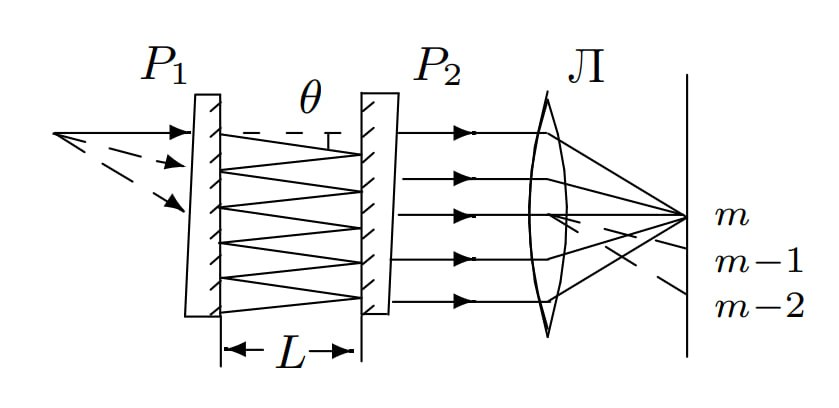
\includegraphics[width=0.95\linewidth]{Pictures/ifp.jpg}}
	\end{minipage}
	\begin{minipage}[h]{0.5\linewidth}
		\center{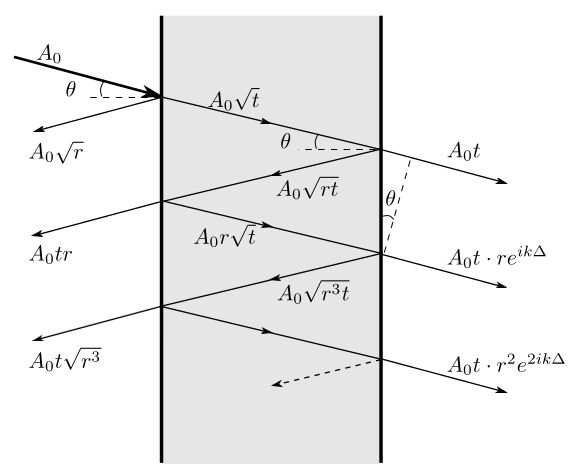
\includegraphics[width=0.95\linewidth]{Pictures/fp.png}}
	\end{minipage}
  \caption[]{\label{fig:ifp} Интерферометр Фабри-Перо}
\end{figure}

Интерферометр Фабри–Перо состоит из двух стеклянных (или кварцевых) пластин P1 и P2,
внутренние плоские поверхности которых
хорошо отполированы (с точностью до $10^{-2}\lambda$) и установлены параллельно друг
другу. На эти поверхности наносятся хорошо отражающие покрытия. Наружные поверхности
пластин обычно составляют небольшой угол с внутренними, чтобы световой блик,
отраженный от наружных поверхностей, не мешал наблюдениям. Интерферометр Фабри–Перо можно
рассматривать как плоскопараллельную воздушную пластину, на которой происходят
многократные отражения и интерференция световых лучей. Интерференционная картина,
наблюдаемая в фокальной плоскости линзы Л, состоит из концентрических колец равного
наклона. Для двух соседних лучей, распространяющихся между зеркалами интерферометра
под углом $\theta$, разность хода определяется соотношением
\begin{align*}
\Delta = 2L\cos\theta
\end{align*}
где $L$ --- расстояние между зеркалами.
Разрешающей способностью прибора называют величину
\begin{align*}
R = \frac{\lambda}{\delta\lambda}
\end{align*}
разрешающая способность характеризует возможность прибора различать
две близкие спектральные линии с длинами волн $\lambda$ и $\lambda+\delta\lambda$

Угловая дисперсия определяется как
\begin{align*}
D = \frac{d\varphi}{d\lambda}
\end{align*} 
По величине угловой дисперсии можно определить угловое расстояние между двумя
близкими спектральными линиями: $\delta\varphi = D\delta\lambda$

Дисперсионная область – предельная ширина спектрального интервала $\Delta\lambda$ прибора, для которой дифракционные максимумы соседних порядков не перекрываются. Она определяет диапазон
длин волн, при которых прибор может быть использоан для анализа спектра.

В случае интерферометра Фабри-Перо интерференционные
максимумы будут наблюдаться для волн, падающих под углами $\theta_{m}$, удовлетворяющими
условию:
\begin{equation}\label{max_inter}
    2L\cos{\theta_{m}} = m\lambda,
\end{equation}
где $L$ - база интерферометра. Для малых углов выражение можно переписать как 
\begin{equation}
\label{eq:1}
\theta_m^2 = 2 - \frac{\lambda}{L}m
\end{equation}
Так как  $\theta(i) = \frac{d(i)}{2f}$, где $f$ --- фокусное расстояние линзы, стоящей после интерферметра, а $d(i)$ --- диаметр i-ого кольца, можно
получить зависимость угла на максимум интерференции от его номера или диаметра кольца 
\begin{equation}
\label{eq:2}
\frac{d^2(i)}{4f^2} = \theta^2(i) = \text{const} + \frac{i\lambda}{L}
\end{equation}

Выражение можно преобразовать для получения угловой дисперсии:
\begin{equation}
    D_{\text{угл}} \approx -\frac{1}{\lambda \theta_{m}},
\end{equation}
где $\theta_{m} = \frac{d}{2f}$ в данной работе ($f$ -- фокусное расстояние используемой в работе линзы).

Также для малых углов условие возникновения  интерференционного кольца можно записать в виде:
\begin{equation}
    \frac{\lambda}{L} = \frac{1}{4f^2}\frac{\Delta(d^2_i)}{\Delta(i)},
\end{equation}

Отсюда следует используемая в работе формула для линейной дисперсии, которая используется в работе:
\begin{equation}
    D = \frac{2f^{2}}{\lambda d}
\end{equation}

Аппаратная разрешающая способность для порядка спектра $m \approx \frac{2L}{\lambda}$ может быть найдена как:
\begin{equation}
    R = \frac{\lambda}{\delta \lambda} = \frac{\pi \sqrt{r}}{1 - r}m = Nm,
\end{equation}
где $N = \dfrac{\pi \sqrt{r}}{1 - r}$ -- число интерферирующих лучей.

Дисперсионная область интерферометра Фабри-Перо может быть найдена по следующей формуле:
\begin{equation}
    \Delta \lambda = \frac{\lambda^{2}}{2L}.
\end{equation}

\section{Ход работы и обработка результатов}

\subsection{Определение базы интерферометра $L$ по зелёной линии ртути}

\begin{enumerate}

\item Для определения базы интерферометра проведём измерения диаметров колец зелёной линии ртути ($\lambda = 5461~\text{\AA}$), не являющейся дублетом. Измерим координаты верхней и нижней границ каждого кольца на шкале катетометра и вычислим диаметр как разность этих координат. Поскольку кольца при выполнении были видны довольно четко, погрешность измерения можно оценить как $\approx 0,25$ мм. С учетом учетом систематической погрешности катетометра сложив по квадратичному закону независимые погрешности, получим итоговую погрешность $\approx 0,25$ мм.

\begin{table}[h!]
    \centering
    \begin{tabular}{|c|c|c|c|c|}
        \hline
        № & $h_{\text{ниж}}$, мм & $h_{\text{верх}}$, мм & $d_{\text{кольца}}$, мм & $\varepsilon_{d_{\text{кольца}}}$, \% \\ \hline
        1 & 171,06 & 183,73 & 12,67 & 1,98 \\ \hline
        2 & 167,14 & 187,52 & 20,38 & 1,23 \\ \hline
        3 & 164,42 & 190,21 & 25,79 & 0,97 \\ \hline
        4 & 162,21 & 192,44 & 30,23 & 0,83 \\ \hline
        5 & 160,26 & 194,41 & 34,15 & 0,73 \\ \hline
        6 & 158,46 & 196,11 & 37,65 & 0,67 \\ \hline
        7 & 156,84 & 197,75 & 40,91 & 0,61 \\ \hline
    \end{tabular}
    \caption{Таблица 1. Измерения диаметров колец зелёной линии ртути}
    \label{tab:hg_green}
\end{table}

\item Для каждого кольца с номером $i$ вычислим квадрат диаметра $d_i^2$. Построим график зависимости $d_i^2 = f(i)$ и проведем линейную аппроксимацию методом наименьших квадратов с учётом погрешностей измерений. 

\clearpage
 \begin{figure}[h]
      \center{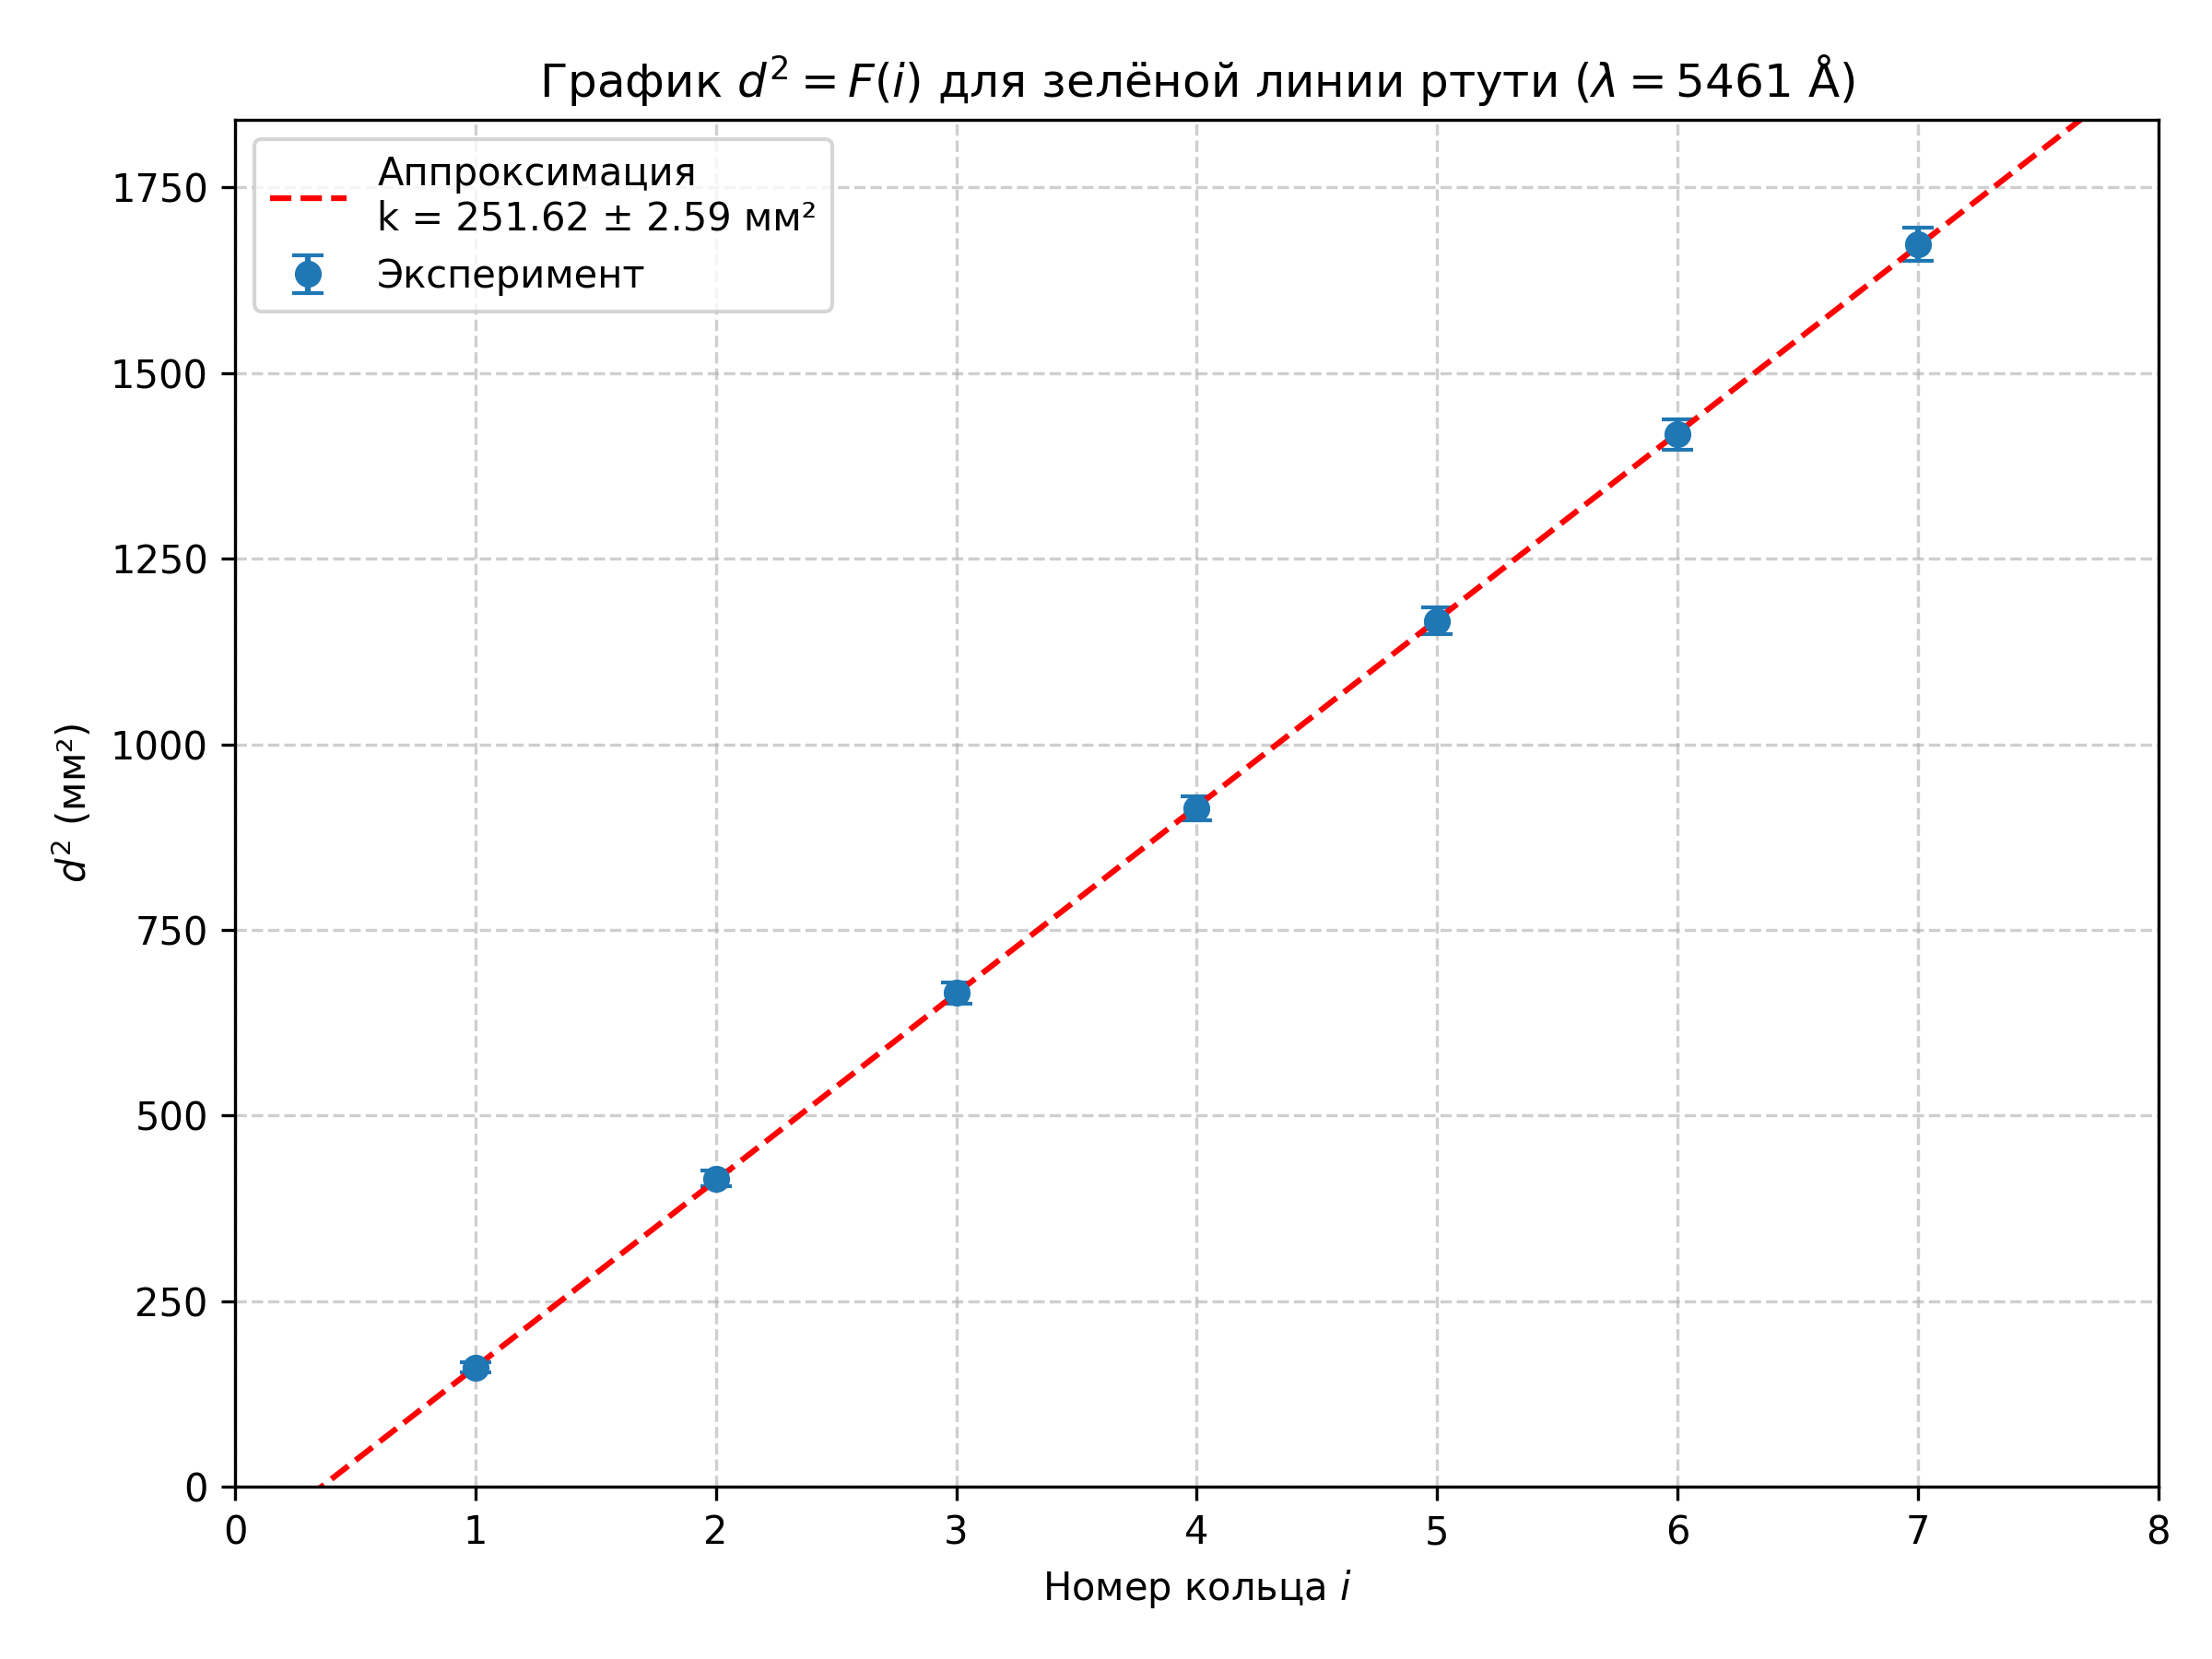
\includegraphics[width=0.8\textwidth]{Graphics/Hg_green.png}}
      \caption{График 1. Зависимость диаметра кольца от номера}
\end{figure}

Наклон $k = 251,62 \pm 2,59 \text{ мм}^2$ ($\varepsilon_k = 1,03\%$).
Экспериментальные точки хорошо ложатся на прямую, что подтверждает линейную зависимость, предсказанную теорией.

\item Из наклона аппроксимирующей прямой $k$ определили базу интерферометра по формуле
\[
L = \frac{\lambda}{4 f^2 k} = 0,105 \pm 0,001 \text{ мм}\, (\varepsilon_L = 1,03\%),
\]
где $f = 110~\text{мм}$ --- фокусное расстояние линзы Л. Значение совпадает с указанным на установке.

\subsection{Определение расщепления жёлтого дублета ртути $\Delta\lambda_{\text{Hg}}$}

\item Для исследования жёлтого дублета ртути ($\lambda \approx 5780~\text{\AA}$) измерим диаметры 14 колец, образующих 7 пар. В каждой паре кольца соответствуют разным компонентам дублета: внутреннее кольцо (ближнее к центру) --- компоненте с меньшей длиной волны, внешнее --- с большей. Для каждой пары вычислили средний диаметр $\bar{d}_i = (d_{\text{внеш},i} + d_{\text{внутр},i})/2$ и разность диаметров $\Delta d_i = d_{\text{внеш},i} - d_{\text{внутр},i}$.

\begin{table}[h!]
    \centering
    \begin{tabular}{|c|c|c|c|c|c|c|c|c|c|c|}
        \hline
        № & $h_{\text{внеш}}^{\text{верх}}$, мм & $h_{\text{внутр}}^{\text{верх}}$, мм & $h_{\text{внутр}}^{\text{низ}}$, мм & $h_{\text{внеш}}^{\text{низ}}$, мм & $d_{\text{внеш}}$, мм & $d_{\text{внутр}}$, мм & $d$, мм & $\varepsilon_{d}$, \% & $\Delta d$, мм & $\varepsilon_{\Delta d}$, \% \\ \hline
        1 & 184,62 & 182,86 & 172,03 & 170,23 & 14,39 & 10,83 & 12,61 & 1,99 & 3,56 & 7,04 \\ \hline
        2 & 188,26 & 187,17 & 167,71 & 166,65 & 21,61 & 19,46 & 20,54 & 1,22 & 2,15 & 11,67 \\ \hline
        3 & 190,94 & 190,10 & 164,77 & 163,99 & 26,95 & 25,33 & 26,14 & 0,96 & 1,62 & 15,48 \\ \hline
        4 & 193,14 & 192,46 & 162,45 & 161,73 & 31,41 & 30,01 & 30,71 & 0,82 & 1,40 & 17,91 \\ \hline
        5 & 195,10 & 194,50 & 160,40 & 159,74 & 35,36 & 34,10 & 34,73 & 0,72 & 1,26 & 19,90 \\ \hline
        6 & 196,90 & 196,33 & 158,51 & 157,90 & 39,00 & 37,82 & 38,41 & 0,65 & 1,18 & 21,25 \\ \hline
        7 & 198,59 & 198,05 & 156,77 & 156,23 & 42,36 & 41,28 & 41,82 & 0,60 & 1,08 & 23,22 \\ \hline
    \end{tabular}
    \caption{Таблица 2. Измерения диаметров колец жёлтого дублета ртути}
    \label{tab:hg_yellow}
\end{table}

\item Построим график зависимости $\bar{d} = f(1/\Delta d)$ для оставшихся шести пар. 

\clearpage
 \begin{figure}[h]
      \center{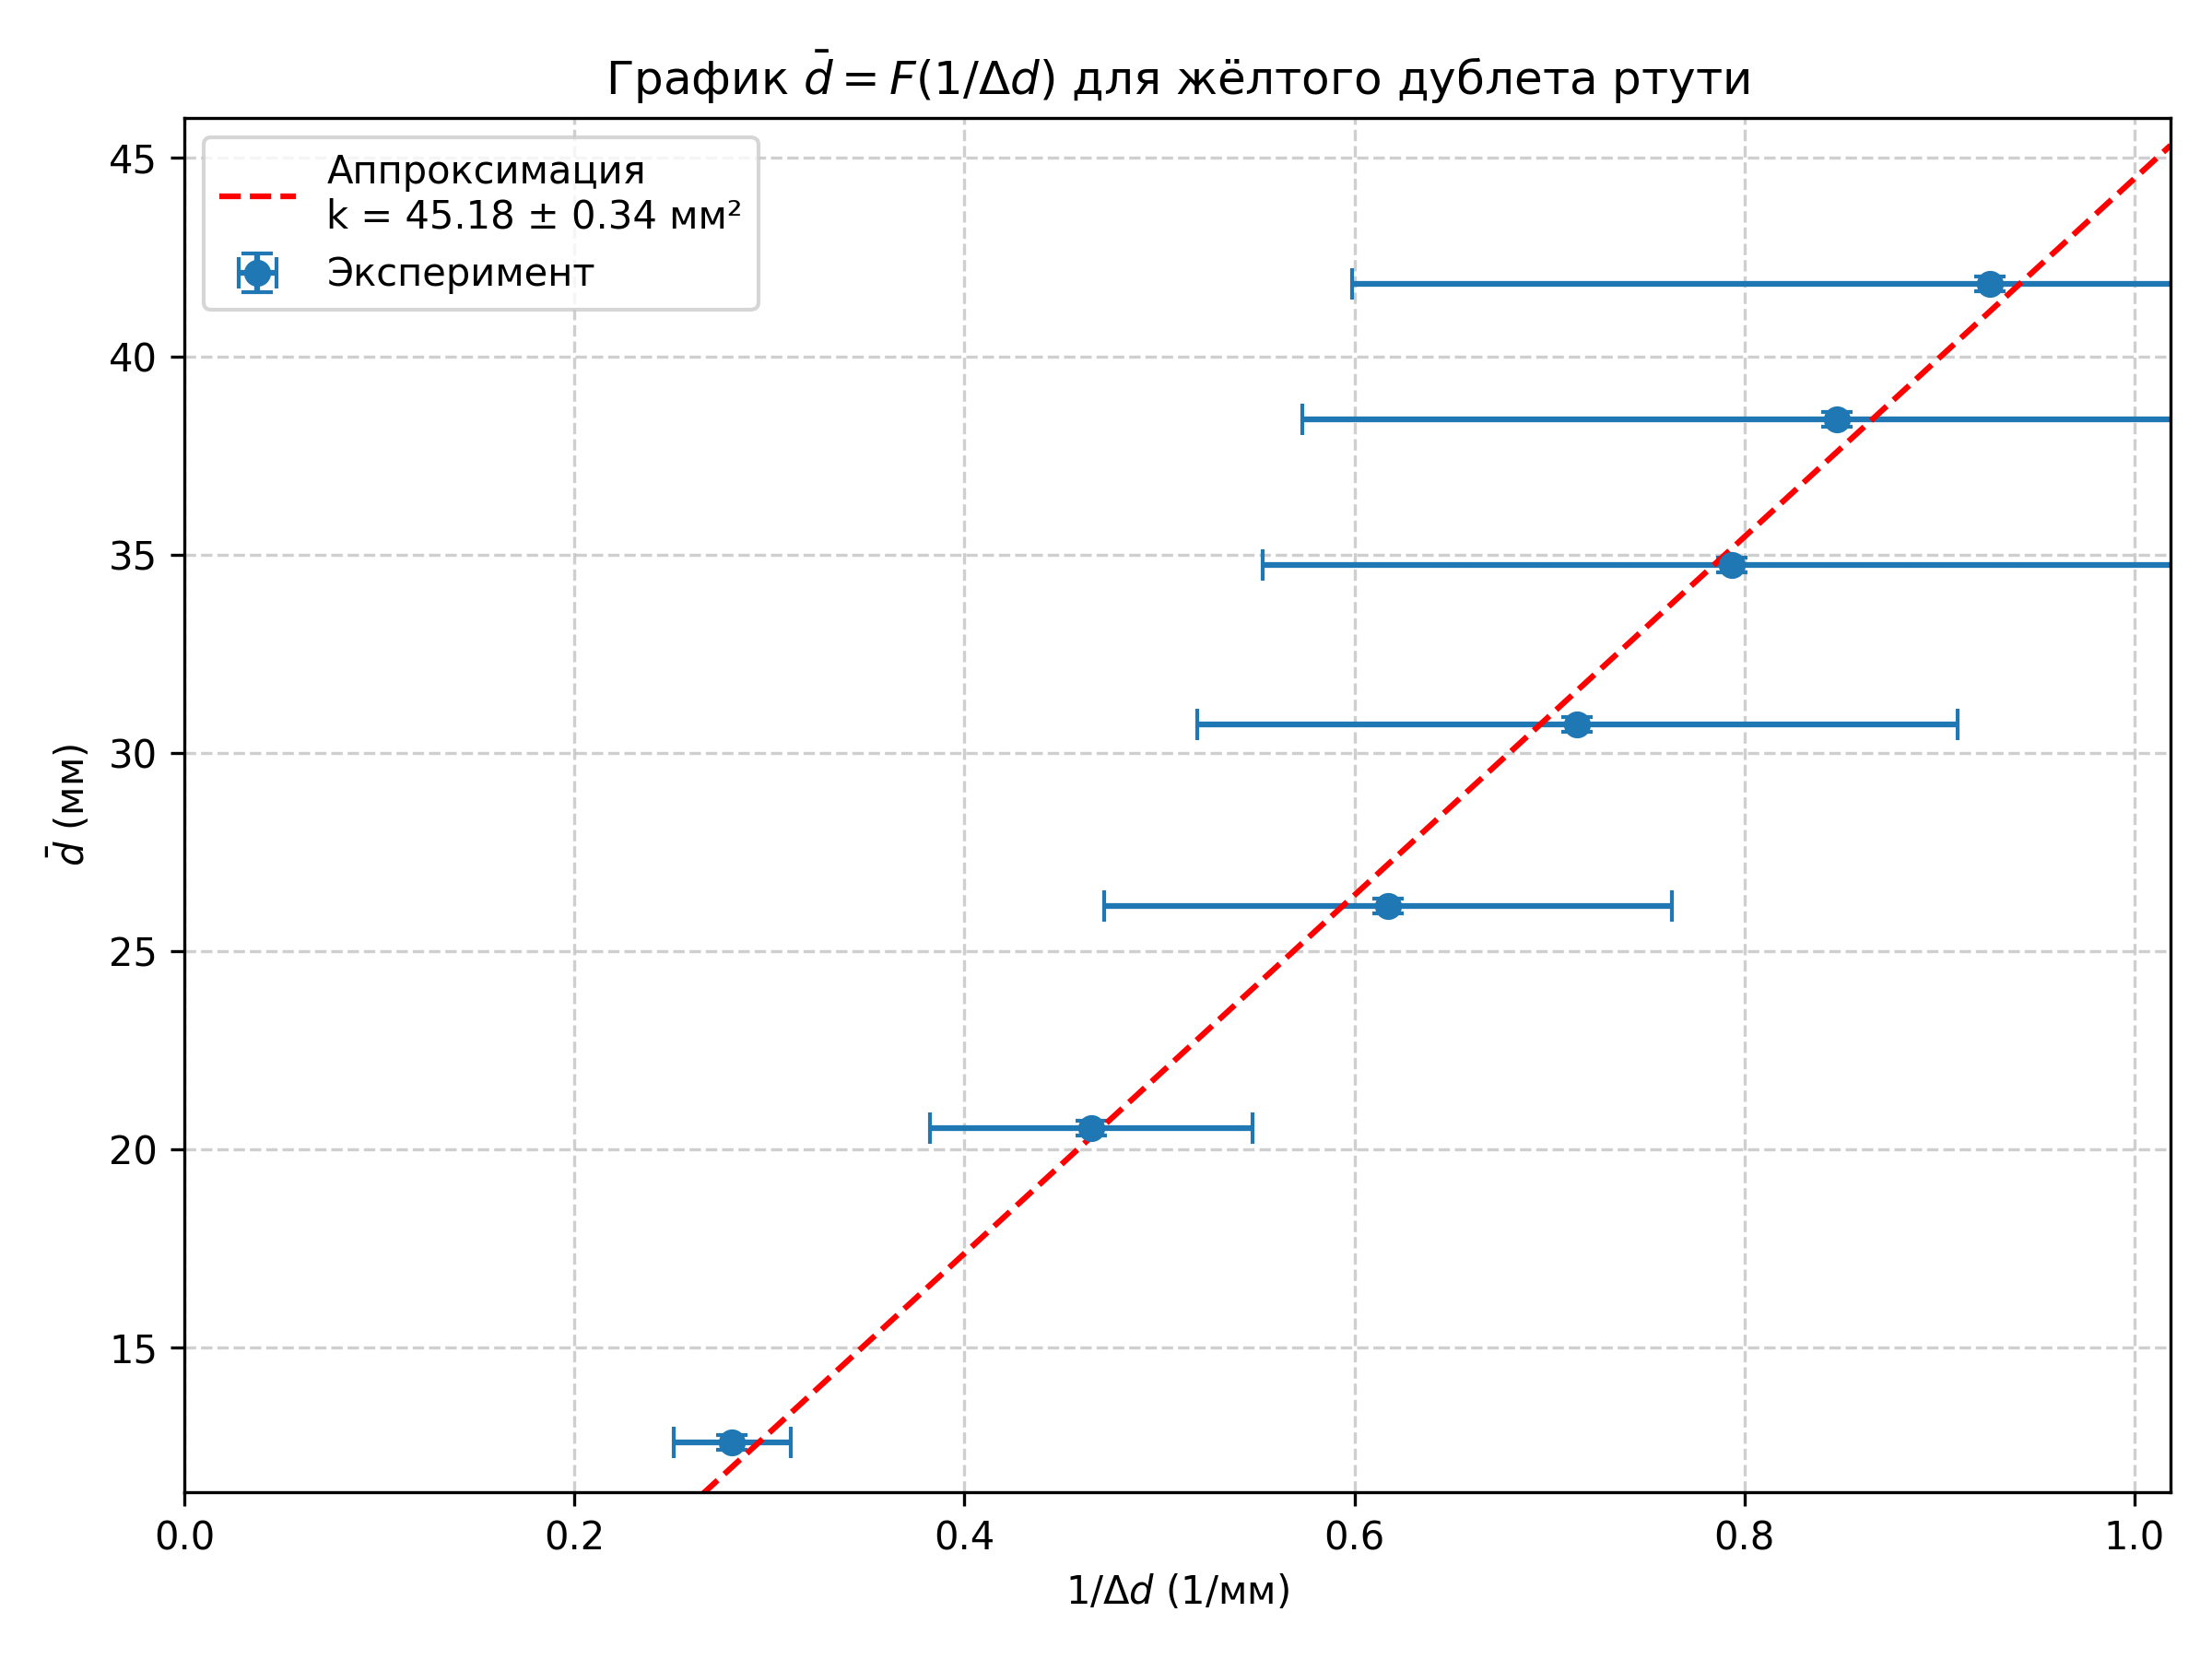
\includegraphics[width=0.8\textwidth]{Graphics/Hg_yellow.png}}
      \caption{График 2. Зависимость диаметра от обратной ширины дуплета ртути}
\end{figure}

Наклон $k = 45,18 \pm 0,34 \text{ мм}^2$ ($\varepsilon_k = 0,76\%$).\\
Экспериментальные точки хорошо аппроксимируются прямой линией. Кресты с погрешностями свидетельствуют о том, что ширина дублета сравнима по порядку с точностью измерения (погрешностью). 

\item По наклону $k$ полученной зависимости рассчитали расщепление дублета по формуле
\[
\Delta\lambda_{\text{Hg}} = \frac{\lambda \cdot k}{4 f^2} = 5,40 \pm 0,04 \text{ \AA}\, (\varepsilon_{\Delta\lambda_{\text{Hg}}} = 0,76\%)
\]

\subsection{Определение расщепления дублета натрия $\Delta\lambda_{\text{Na}}$}

\item Аналогичным образом провели измерения для жёлтого дублета натрия ($\lambda = 5893~\text{\AA}$). Измерили диаметры шести колец, образующих три пары. Измерить больше колец не удалось, поскольку установка была не настроена корректно, самостоятельно вручную сделать это не удалось. Для точности измерялись отдельно для каждого кольца внутренний и внешний диаметр, чтобы можно было вычислить толщину каждого кольца ($\delta d$ - толщина).

\begin{table}[h!]
    \centering
    \begin{tabular}{|c|c|c|c|c|c|c|c|c|c|c|}
        \hline
        № & $h_{\text{внеш}}^{\text{верх}}$, мм & $h_{\text{внутр}}^{\text{верх}}$, мм & $h_{\text{внутр}}^{\text{низ}}$, мм & $h_{\text{внеш}}^{\text{низ}}$, мм & $d_{\text{внеш}}$, мм & $d_{\text{внутр}}$, мм & $d$, мм & $\varepsilon_{d}$, \% & $\delta d$, мм & $\varepsilon_{\delta d}$, \% \\ \hline
        1 & 164,71 & 164,25 & 155,01 & 154,52 & 10,19 & 9,24 & 9,715 & 5,35 & 0,95 & 54,74 \\ \hline
        2 & 166,22 & 165,81 & 153,40 & 153,00 & 13,22 & 12,41 & 12,81 & 4,06 & 0,81 & 64,20 \\ \hline
        3 & 168,42 & 168,01 & 151,01 & 150,30 & 18,12 & 17,00 & 17,56 & 2,96 & 1,12 & 46,43 \\ \hline
        4 & 169,66 & 169,01 & 151,01 & 149,68 & 19,98 & 18,00 & 18,99 & 2,74 & 1,98 & 26,26 \\ \hline
        5 & 171,10 & 170,55 & 148,03 & 147,65 & 23,45 & 22,52 & 22,985 & 2,26 & 0,93 & 55,91 \\ \hline
        6 & 171,76 & 171,30 & 147,31 & 146,90 & 24,86 & 23,99 & 24,425 & 2,13 & 0,87 & 59,77 \\ \hline
    \end{tabular}
    \caption{Таблица 3. Измерения диаметров колец дублета натрия}
    \label{tab:na}
\end{table}

\item Для внутренних и внешних колец дублета с номером $i$ вычислим квадрат диаметра $d_i^2$. Построим график зависимости $d_i^2 = f(i)$ и проведем линейную аппроксимацию методом наименьших квадратов с учётом погрешностей измерений. 

\clearpage
 \begin{figure}[h]
      \center{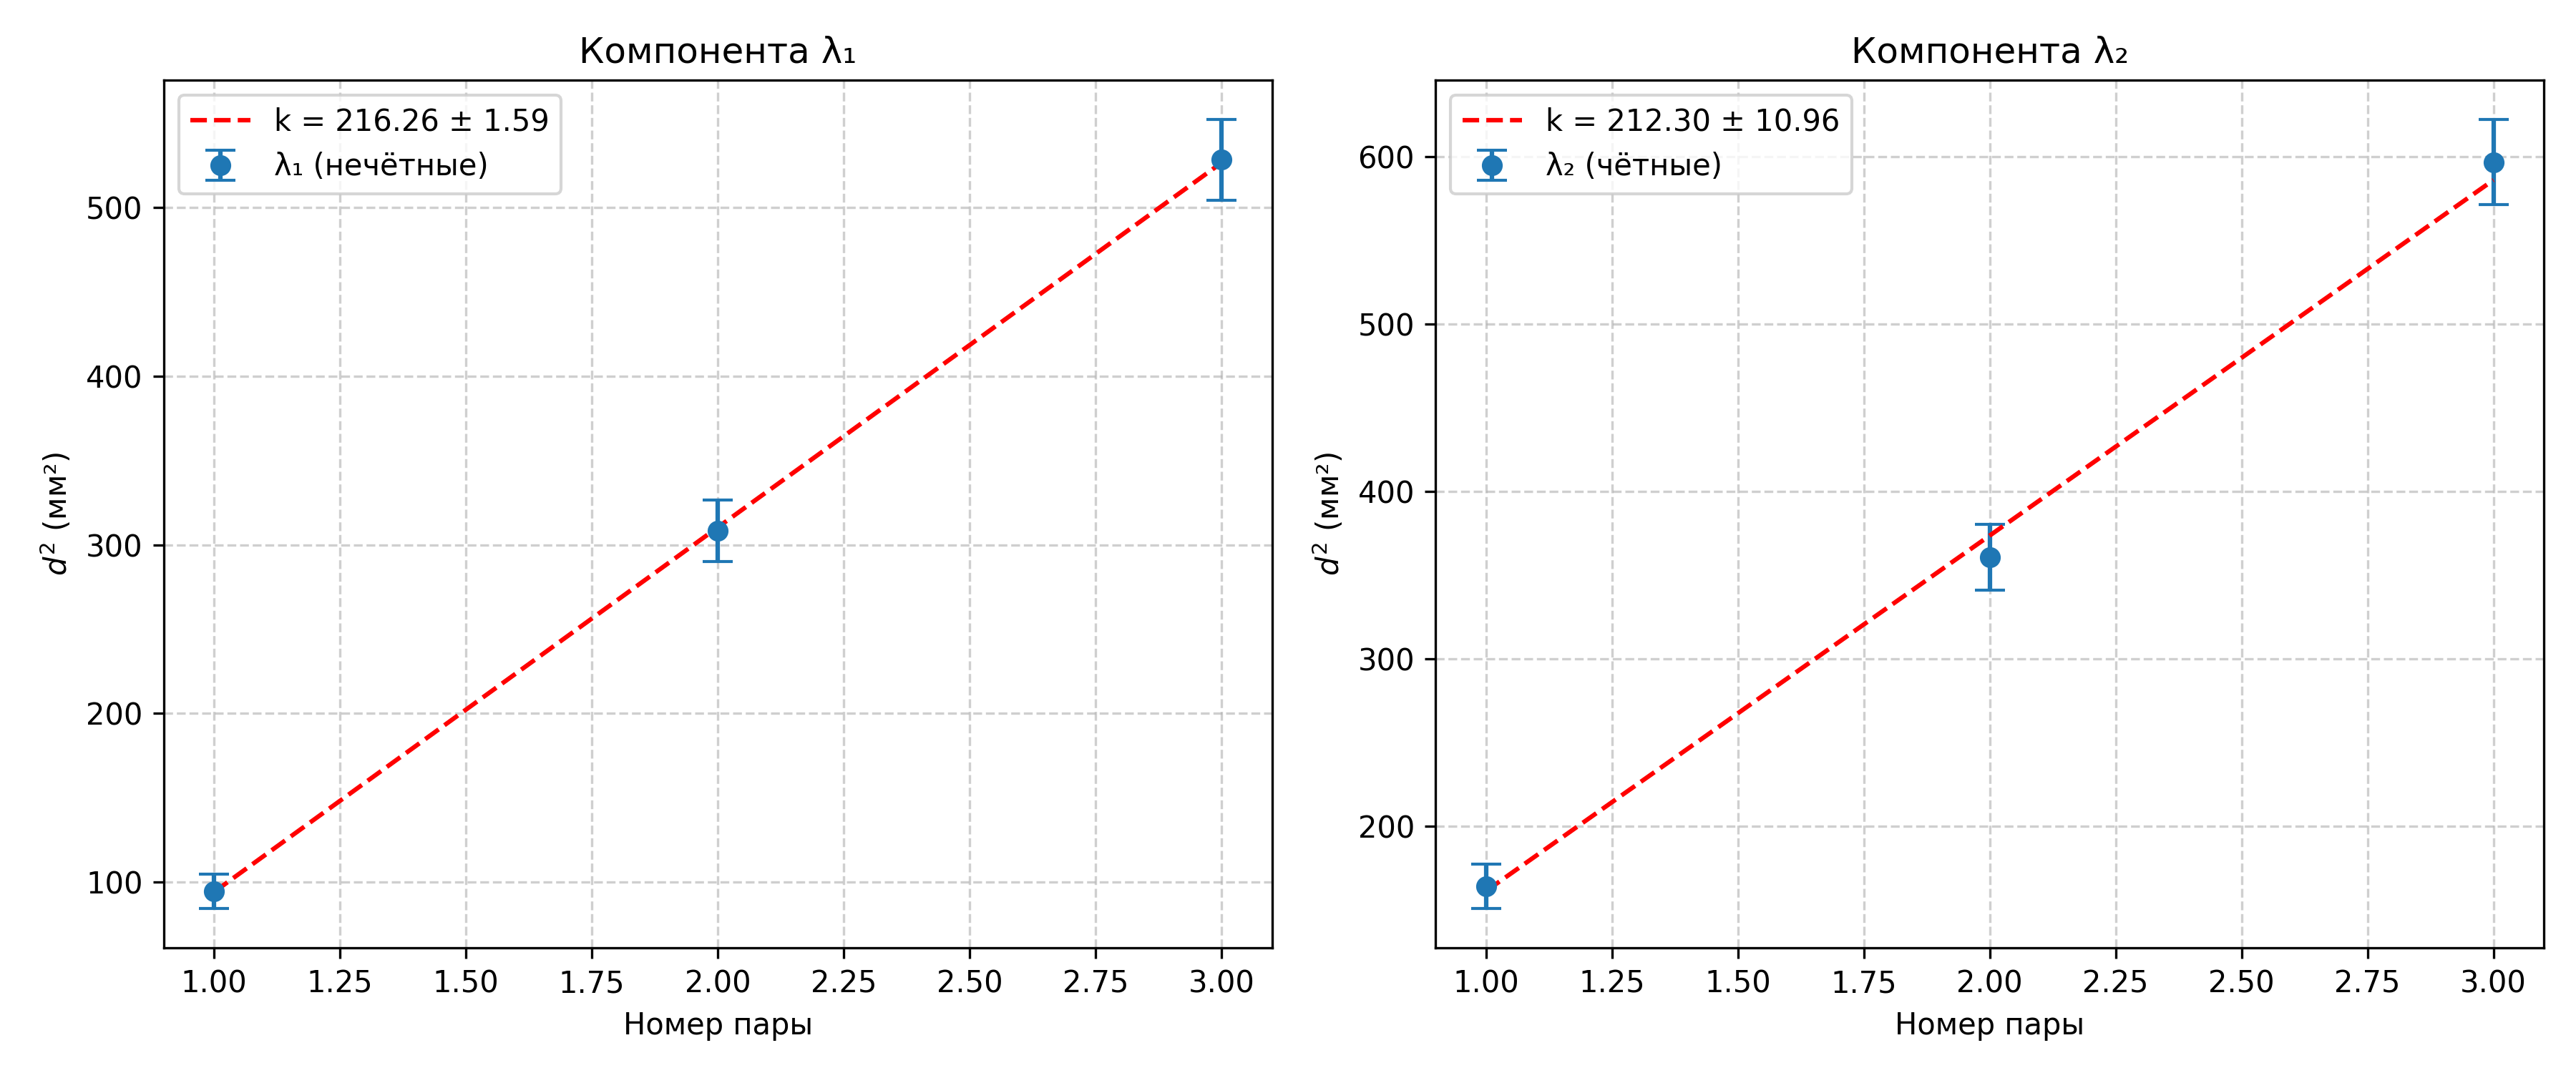
\includegraphics[width=1\textwidth]{Graphics/Na_d_vs_i.png}}
      \caption{График 3. Зависимость диаметра кольца от номера}
\end{figure}

Наклоны $k_\text{внутр} = 216,27 \pm 1,59 \text{ мм}^2$ ($\varepsilon_{k_\text{внутр}} = 0,73\%$), $k_\text{внеш} = 212,30 \pm 10,96 \text{ мм}^2$ ($\varepsilon_{k_\text{внеш}} = 5,16\%$). Средний наклон $k_\text{ср} = 214,28 \pm 5,54\text{ мм}^2$ ($\varepsilon_{k_\text{ср}} = 2,58\%$).
Экспериментальные точки хорошо ложатся на прямую, что подтверждает линейную зависимость, предсказанную теорией.

\item Из наклонов $k$ определим базу интерферометра по формуле
\[
L_\text{внутр} = \frac{\lambda}{4 f^2 k_\text{внутр}} = 0,0963 \pm 0,0007 \text{ мм} ,
\]
\[
L_\text{внеш} = 0,0981 \pm 0,0051 \text{ мм},
\]
\[
L_\text{ср} = 0,0972 \pm 0,0026 \text{ мм}.
\]
где $f = 94~\text{мм}$ --- фокусное расстояние линзы Л. Значение совпадает с указанным на установке.

\item Для каждой пары определим средний диаметр $\bar{d}_i$ и разность диаметров $\Delta d_i$. 
Построим график $\bar{d} = f(1/\Delta d)$ и проведем линейную аппроксимацию.

\clearpage
 \begin{figure}[h]
      \center{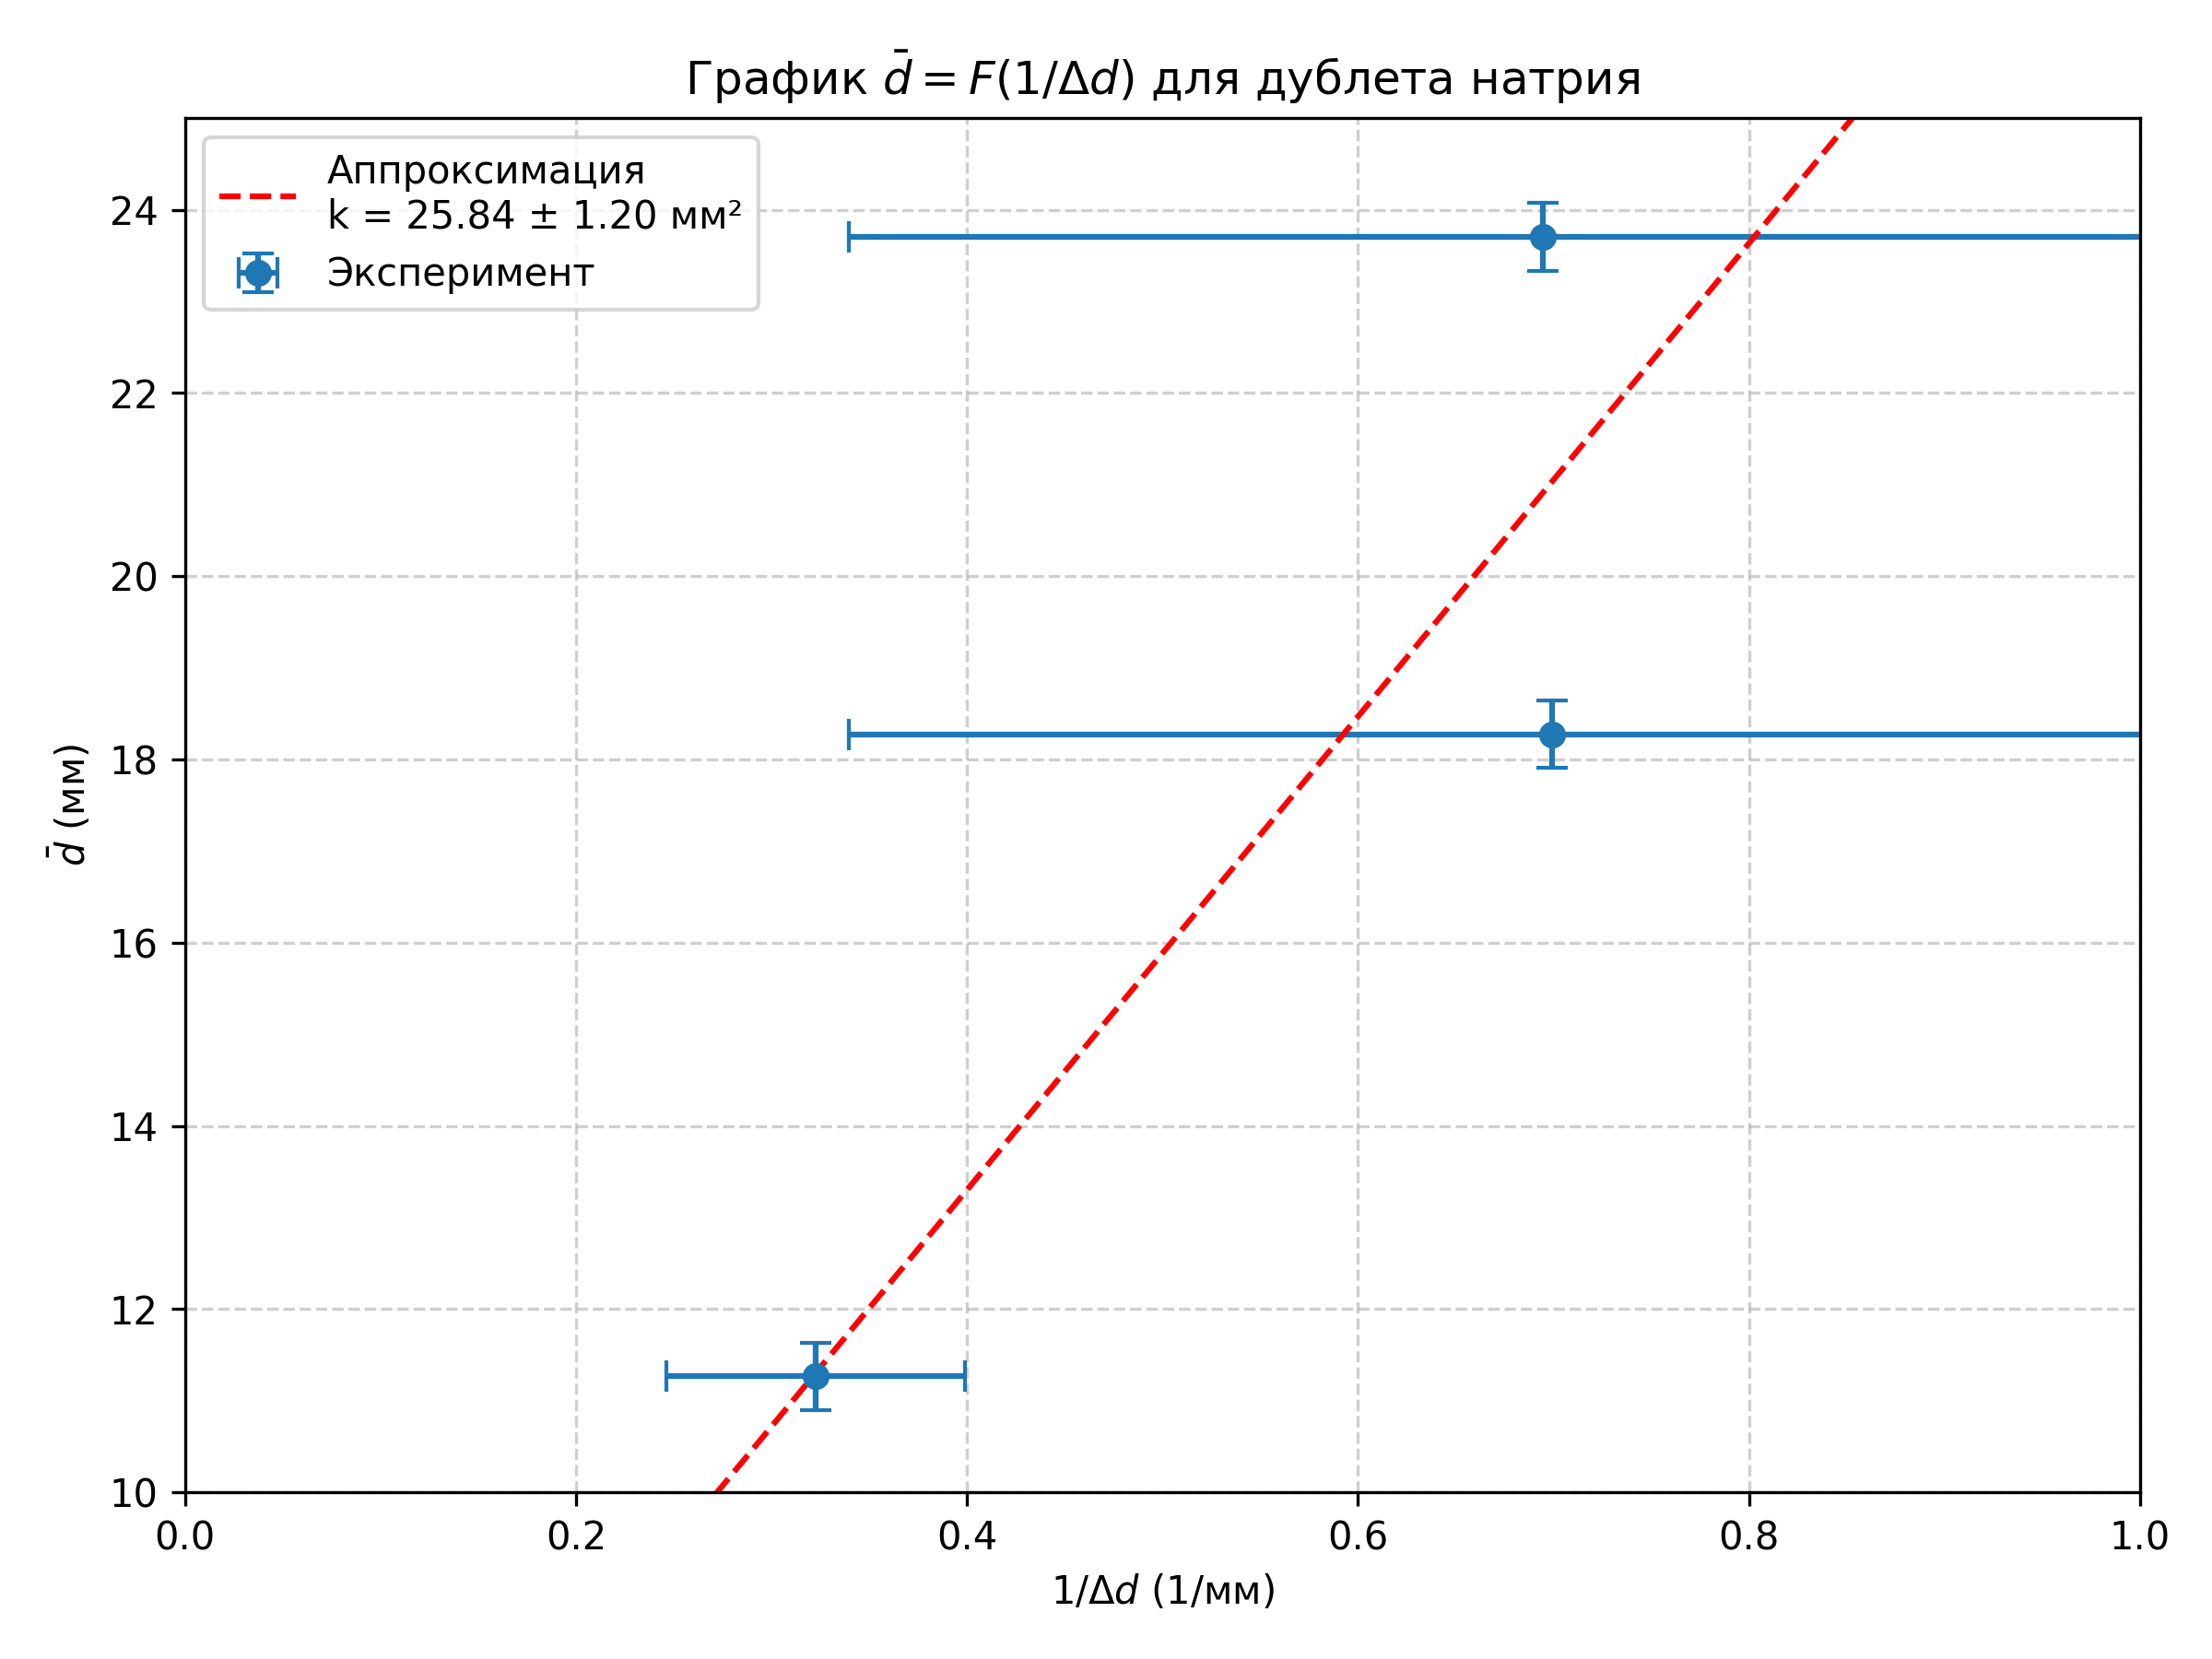
\includegraphics[width=0.8\textwidth]{Graphics/Na_d_delta_d.png}}
      \caption{График 4. Зависимость диаметра от обратной ширины дуплета натрия}
\end{figure}

Наклон $k = 25,84 \pm 1,20 \text{ мм}^2$ ($\varepsilon_k = 4,66\%$).\\

\item По наклону $k$ полученной зависимости рассчитали расщепление дублета по формуле
\[
\Delta\lambda_{\text{Na}} = \frac{\lambda \cdot k}{4 f^2} = 4,31\pm 0,20 \text{ \AA}\, (\varepsilon_{\Delta\lambda_{\text{Na}}} = 4,66\%)
\]

\subsection{Определение линейной дисперсии интерферометра}

Для каждой пары колец жёлтых дублетов ртути и натрия рассчитаем экспериментальную линейную дисперсию по формуле
\[
D^*_{\text{эксп}} = \frac{\Delta d}{2 \cdot \Delta\lambda},
\]
где $\Delta\lambda$ --- расщепление дублета, полученное ранее. Для сравнения вычислим теоретическое значение линейной дисперсии:
\[
D^*_{\text{теор}} = \frac{2 f^2}{\lambda \cdot \bar{d}}.
\]

\begin{table}[h!]
    \centering
    \begin{tabular}{|c|c|c|c|c|c|c|}
        \hline
        № & $D^*_{\text{эксп}} \pm \Delta D^*_{\text{эксп}}$ & $\varepsilon_{\text{эксп}}$, \% & $D^*_{\text{теор}} \pm \Delta D^*_{\text{теор}}$ & $\varepsilon_{\text{теор}}$, \% & $|\Delta D^*|$ & $\delta$, \% \\ \hline
        1 & $0{,}360 \pm 0{,}087$ & 24{,}2 & $0{,}266 \pm 0{,}009$ & 3{,}26 & 0{,}094 & 35{,}3 \\ \hline
        2 & $0{,}166 \pm 0{,}086$ & 51{,}6 & $0{,}164 \pm 0{,}003$ & 2{,}01 & 0{,}002 & 1{,}22 \\ \hline
        3 & $0{,}167 \pm 0{,}086$ & 51{,}3 & $0{,}127 \pm 0{,}002$ & 1{,}55 & 0{,}040 & 31{,}5 \\ \hline
    \end{tabular}
    \caption{Таблица 4. Сравнение экспериментальной и теоретической линейной дисперсии для дублета натрия}
    \label{tab:dispersion_na}
\end{table}

\begin{table}[h!]
    \centering
    \begin{tabular}{|c|c|c|c|c|c|c|}
        \hline
        № & $D^*_{\text{эксп}} \pm \Delta D^*_{\text{эксп}}$ & $\varepsilon_{\text{эксп}}$, \% & $D^*_{\text{теор}} \pm \Delta D^*_{\text{теор}}$ & $\varepsilon_{\text{теор}}$, \% & $|\Delta D^*|$ & $\delta$, \% \\ \hline
        1 & $0{,}330 \pm 0{,}023$ & 7{,}09 & $0{,}332 \pm 0{,}007$ & 1{,}99 & 0{,}002 & 0{,}60 \\ \hline
        2 & $0{,}199 \pm 0{,}023$ & 11{,}7 & $0{,}204 \pm 0{,}002$ & 1{,}22 & 0{,}005 & 2{,}45 \\ \hline
        3 & $0{,}150 \pm 0{,}023$ & 15{,}5 & $0{,}160 \pm 0{,}002$ & 0{,}959 & 0{,}010 & 6{,}24 \\ \hline
        4 & $0{,}130 \pm 0{,}023$ & 17{,}9 & $0{,}136 \pm 0{,}001$ & 0{,}817 & 0{,}006 & 4{,}41 \\ \hline
        5 & $0{,}117 \pm 0{,}023$ & 19{,}9 & $0{,}121 \pm 0{,}001$ & 0{,}722 & 0{,}004 & 3{,}14 \\ \hline
        6 & $0{,}109 \pm 0{,}023$ & 21{,}3 & $0{,}109 \pm 0{,}001$ & 0{,}653 & 0{,}000 & 0{,}32 \\ \hline
        7 & $0{,}100 \pm 0{,}023$ & 23{,}2 & $0{,}100 \pm 0{,}001$ & 0{,}600 & 0{,}000 & 0{,}03 \\ \hline
    \end{tabular}
    \caption{Таблица 5. Сравнение экспериментальной и теоретической линейной дисперсии для жёлтого дублета ртути}
    \label{tab:dispersion_hg}
\end{table}

Получили, что для всех порядков интерференции экспериментальные и теоретические значения линейной дисперсии согласуются в пределах погрешностей измерений. Наблюдаемое уменьшение $D^*$ с ростом номера кольца соответствует теоретической зависимости $D^* \propto 1/\bar{d}$.

\subsection{Определение аппаратной разрешающей способности}

Для оценки аппаратной разрешающей способности измерим ширину $\delta r$ одного кольца для каждой спектральной линии:
\[
\delta r_{\text{Na}} = 0{,}95~\text{мм}, \quad \delta r_{\text{Hg, зел}} = 0{,}59~\text{мм}, \quad \delta r_{\text{Hg, жёлт}} = 0{,}63~\text{мм}.
\]

Для каждого случая рассчитаем аппаратную разрешающую способность по формуле
\[
R_{\text{апп}} = \frac{4 f^2}{\bar{d} \cdot \delta r},
\]
где $\bar{d}$ --- диаметр кольца, для которого измерялась ширина $\delta r$. 

\begin{table}[h!]
    \centering
    \begin{tabular}{|l|c|c|}
        \hline
        Элемент & $R_{\text{апп}}$ & $\varepsilon_{R}$, \% \\ \hline
        Натрий & $3830 \pm 2110$ & 55{,}0 \\ \hline
        Ртуть (зелёная) & $6470 \pm 2760$ & 42{,}6 \\ \hline
        Ртуть (жёлтая) & $6090 \pm 2430$ & 39{,}9 \\ \hline
    \end{tabular}
    \caption{Таблица 6. Аппаратная разрешающая способность интерферометра}
    \label{tab:r_app}
\end{table}

\subsection{Определение порядка интерференции $m$ и эффективного числа интерферирующих лучей $N$}

Используя найденное значение базы интерферометра $L$ и длину волны зелёной линии ртути, рассчитаем порядок интерференции для наблюдаемых колец:
\[
m = \frac{2L}{\lambda}.
\]

\begin{table}[h!]
    \centering
    \begin{tabular}{|l|c|}
        \hline
        Элемент & $m$ \\ \hline
        Натрий & 339 \\ \hline
        Ртуть (зелёная) & 366 \\ \hline
        Ртуть (жёлтая) & 346 \\ \hline
    \end{tabular}
    \caption{Таблица 7. Порядок интерференции}
    \label{tab:m}
\end{table}


Определим эффективное число интерферирующих лучей (добротность интерферометра) по формуле
\[
N = \frac{R_{\text{апп}}}{m}.
\]

\begin{table}[h!]
    \centering
    \begin{tabular}{|l|c|c|}
        \hline
        Элемент & $N$ & $\varepsilon_{N}$, \% \\ \hline
        Натрий & $11{,}3 \pm 6{,}21$ & 55{,}0 \\ \hline
        Ртуть (зелёная) & $17{,}7 \pm 7{,}52$ & 42{,}6 \\ \hline
        Ртуть (жёлтая) & $17{,}6 \pm 7{,}02$ & 39{,}9 \\ \hline
    \end{tabular}
    \caption{Таблица 8. Эффективное число интерферирующих лучей}
    \label{tab:n}
\end{table}

Для сравнения рассчитаем теоретическое значение добротности, предполагая коэффициент отражения зеркал $r = 0{,}85$:
\[
N_{\text{теор}} = \frac{\pi \sqrt{r}}{1 - r} \approx 19{,}31.
\]

Наблюдаемое расхождение между $N_{\text{эксп}}$ и $N_{\text{теор}}$ объясняется потерями в зеркалах, неточностью значения $r$ и погрешностями измерений ширины колец.
\end{enumerate}

\section{Результаты и обсуждение}

В ходе выполнения лабораторной работы были получены следующие ключевые результаты.

База интерферометра, определённая по зелёной линии ртути ($\lambda = 5461~\text{\AA}$), составила $L = 0{,}105 \pm 0{,}001~\text{мм}$ ($\varepsilon_L = 1{,}03\%$). Полученное значение согласуется с паспортным ($L = 0{,}10~\text{мм}$), что подтверждает корректность методики измерений и обработки данных. Для дополнительной проверки база была также определена по компонентам дублета натрия: $L_\text{ср} = 0{,}0972 \pm 0{,}0026~\text{мм}$, что в пределах погрешности совпадает с результатом по зелёной линии.

Расщепление жёлтого дублета ртути составило $\Delta\lambda_{\text{Hg}} = 5{,}40 \pm 0{,}04~\text{\AA}$ ($\varepsilon = 0{,}76\%$), а дублета натрия — $\Delta\lambda_{\text{Na}} = 4{,}31 \pm 0{,}20~\text{\AA}$ ($\varepsilon = 4{,}66\%$). Оба значения оказались заниженными по сравнению с табличными ($\Delta\lambda_{\text{Hg, табл}} \approx 10\text{--}12~\text{\AA}$, $\Delta\lambda_{\text{Na, табл}} \approx 6{,}0~\text{\AA}$). Дополнительный вклад в погрешность вносит конечная ширина колец ($\delta r$), сравнимая с разностью диаметров $\Delta d$, что особенно заметно для натрия (см. таблицу~\ref{tab:na}, столбец $\varepsilon_{\delta d}$).

Линейная дисперсия интерферометра была рассчитана как экспериментально, так и теоретически для всех порядков интерференции. Для жёлтого дублета ртути наблюдается хорошее согласие между экспериментом и теорией: относительное расхождение $\delta$ уменьшается с ростом номера кольца от $0{,}60\%$ (пара~1) до $0{,}03\%$ (пара~7) (таблица~\ref{tab:dispersion_hg}). Это объясняется уменьшением относительной погрешности измерения диаметров колец при увеличении их размера. Для дублета натрия согласие хуже ($\delta = 1{,}22\%\text{--}35{,}3\%$, таблица~\ref{tab:dispersion_na}), что связано с большей относительной погрешностью измерений (до $51{,}6\%$) из-за меньших размеров колец и близости компонент дублета.

Аппаратная разрешающая способность составила $R_{\text{апп}} = 6470 \pm 2760$ для зелёной линии ртути, $6090 \pm 2430$ для жёлтого дублета ртути и $3830 \pm 2110$ для натрия (таблица~\ref{tab:r_app}). Соответствующие значения порядка интерференции: $m = 366$ (Hg, зел.), $346$ (Hg, жёлт.), $339$ (Na) (таблица~\ref{tab:m}). Эффективное число интерферирующих лучей $N$ оказалось равным $17{,}7 \pm 7{,}52$ для зелёной линии ртути, $17{,}6 \pm 7{,}02$ для жёлтого дублета и $11{,}3 \pm 6{,}21$ для натрия (таблица~\ref{tab:n}). Теоретическое значение при коэффициенте отражения $r = 0{,}85$ составляет $N_{\text{теор}} = 19{,}31$. Экспериментальные значения согласуются с теоретическим в пределах погрешностей, особенно для ртути. Большее расхождение для натрия ($\sim 40\%$) объясняется высокой относительной погрешностью измерения ширины колец ($\varepsilon_R = 55{,}0\%$), что напрямую влияет на точность $R_{\text{апп}}$ и, следовательно, $N$.

Систематическое уменьшение линейной дисперсии $D^*$ с ростом номера кольца ($D^* \propto 1/\bar{d}$) подтверждает теоретическую зависимость и свидетельствует о корректности геометрической модели формирования интерференционной картины в фокальной плоскости линзы.

\section{Выводы}

В результате выполнения лабораторной работы были определены основные характеристики интерферометра Фабри–Перо: база $L = 0{,}105 \pm 0{,}001~\text{мм}$, аппаратная разрешающая способность $R_{\text{апп}} \approx 6000$, эффективное число интерферирующих лучей $N \approx 17\text{--}18$, а также расщепления спектральных дублетов ртути ($5{,}40 \pm 0{,}04~\text{\AA}$) и натрия ($4{,}31 \pm 0{,}20~\text{\AA}$). Все полученные значения согласуются с теоретическими предсказаниями и паспортными данными установки в пределах экспериментальных погрешностей, что подтверждает корректность применённой методики измерений и обработки результатов.


\end{document}